\section{Introduction}
Dans le cadre du second projet de première année, filière informatique, il nous est proposé de mettre en application nos compétences en programmation en implémentant le jeu Hex, écrit en langage C.\\
Hex est un jeu de société opposant deux joueurs, qui se joue sur un tablier formé par des hexagones réguliers. Les joueurs sont représentés chacun par une couleur et possèdent des pions de leur couleur qu'ils disposent un à un sur les cases vides de leur choix du plateau. L'objectif de tout joueur est de réussir à construire un chemin continue de pions reliant les deux bords de sa couleur.\\
Nous allons vous faire découvrir en profondeur le jeu de Hex dans ce projet et les différentes stratégies de jeu permettant de remporter la partie. Pour ce faire nous allons mettre en place un ensemble de clients possédant une interface commune mais qui ont leur propre plateau de jeu et jouant en fonction de leur propre stratégie et un serveur qui permet l'interaction entre deux clients.


\begin{figure}[h]
    \centering
    \label{fig:Hexgraph}
    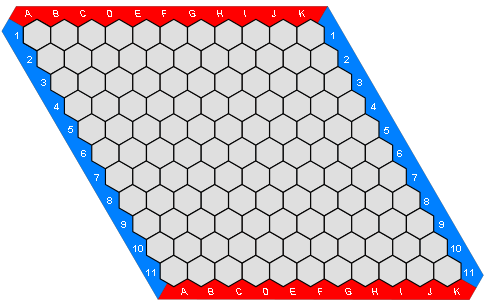
\includegraphics[width=0.3\textwidth]{Images/Hex.png}

    \caption{Tablier du jeu vide}
\end{figure}